\RequirePackage{luatex85}
\documentclass[tikz,border=0]{standalone}
\usepackage[no-math]{fontspec}
\setmainfont[Ligatures=TeX]{PragmataPro-Bold}
\usetikzlibrary{positioning,backgrounds,fit,shapes.geometric,calc}
\usepackage{pgfplots}
\definecolor{bgColor}{RGB}{38,50,56}
\definecolor{textColor}{RGB}{195,206,227}
\definecolor{edgeColor}{RGB}{125,198,191}
\begin{document}
  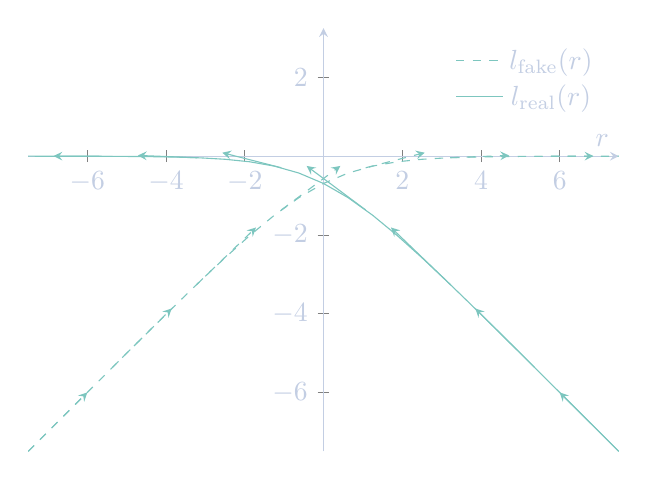
\begin{tikzpicture}[textColor]
    \begin{axis}[
      axis lines=center,axis on top=false,scale only axis=true,
      samples=25,domain=-7.5:7.5,
      x=.5cm,xmin=-7.5,xmax=7.5,
      xlabel=$r$,
      y=.5cm,ymin=-7.5,ymax=3.25,
      legend style={draw=none,fill=none},
      legend entries={$l_{\mathrm{fake}}(r)$,$l_{\mathrm{real}}(r)$}
    ]
      \addplot [edgeColor,dashed] {- ln(1 + exp(-x))};
      \addplot [edgeColor] {- ln(1 + exp(x))};
      \addplot [edgeColor,quiver={u=-1.5,v=1.5/(1+exp(-x))},-stealth,samples=8] {- ln(1 + exp(x))};
      \addplot [edgeColor,dashed,quiver={u=1.5,v=1.5/(1+exp(x))},-stealth,samples=8] {- ln(1 + exp(-x))};
    \end{axis}
  \end{tikzpicture}
\end{document}